\documentclass[pss]{wiley2sp} % provides pss two-column style
\usepackage{amsmath}
\usepackage{subfig}

\renewcommand{\arraystretch}{1.2} % please do not remove or change
\tolerance=400
\emergencystretch=10pt

\begin{document}


% Title of the article
\title{Nonlinear optical responses in hydrogenated graphene structures}

% Authors
\author{
Reinaldo Zapata-Pe\~na\textsuperscript{\Ast,\textsf{\bfseries 1}},
Sean M. Anderson\textsuperscript{\Ast,\textsf{\bfseries 1}},
Bernardo S. Mendoza\textsuperscript{\Ast,\textsf{\bfseries 1}},
Anatoli I. Shkrebtii\textsuperscript{\textsf{\bfseries 2}}}

% Abbreviated list of authors for the page headers
\titlerunning{Optical spin injection, current injection, and SHG study of
hydrogenated graphene}
\authorrunning{R. Zapata-Pe\~na et al.}

%E-mail-address of corresponding author
\mail{e-mail
  \textsf{bms@cio.mx}, Phone:
  +52-477-441-4200, Fax: +52-477-441-4209}

% author's affiliations/addresses
\institute{%
  \textsuperscript{1}\,Centro de Investigaciones en \'Optica, Le\'on,
  Guanajuato 37150, M\'exico\\
  \textsuperscript{2}\,University of Ontario, Institute of Technology, Oshawa,
  ON, L1H 7L7, Canada}

\received{XXXX, revised XXXX, accepted XXXX}
\published{XXXX} % do not change, will be filled in by the publisher

% Please select about four verbal keywords for your manuscript.
\keywords{graphene, spin polarization, current injection, second-harmonic.}

\abstract{%
\abstcol{%
We present a theoretical study of the optical spin injection, optical current
injection, and second harmonic generation of two 50\% hydrogenated graphene
structures: C$_{16}$H$_{8}$-alt and C$_{16}$H$_{8}$-up. Optical spin
injection, under incidence of circularly polarized light into nonmagnetic
semiconductors, creates spin-polarized electrons in the conduction bands. The
optical current injection and second-harmonic generation are nonlinear
second-order effects that are allowed in materials without inversion symmetry.}
{The results are calculated in a full electronic band structure scheme within
DFT in the LDA approximation. Our results show an anisotropic behavior of the
spin and current injection and second harmonic generation optical response. We
obtain maximum absolute magnitudes of the degree of spin polarization of 61\%
and 64\% for the \emph{alt} and \emph{up} structures, respectively. It is also
possible to optically generate injection current coming mainly from the carbon
layer on both \emph{alt} and \emph{up} systems. Also we found that both
structures are excellent candidates for second harmonic generation.}}

\maketitle


\section{Introduction}\label{sec:intro}

Graphene is an allotrope of carbon with a planar, hexagonal, two-dimensional
honeycomb structure with one carbon atom at each vertex, as shown in Fig.
\ref{fig:structures}. It has attracted a great deal of interest due to its
distinctive properties, such as the fractional quantum Hall effect at room
temperature, and excellent thermal transport properties
\cite{geimNM07,reinaNL08,novoselov2S7,balandinNL08}. It behaves like a metal,
but can be modified to semiconductor behavior by tuning the band gap. This can
be achieved by changing the surface area \cite{hanPRL07}, applying an electric
field \cite{zhangN09}, applying uniaxial strain \cite{niACSN08}, or by doping,
amongst other methods. Previous works have explored doping with boron,
nitrogen \cite{guoIJ11}, and hydrogen
\cite{eliasS09,guisingerNL09,samarakoonACSN10}.

Hydrogenated graphene can obtain different spatial configurations by varying
the amount and location of the hydrogen bonds. In this paper we present a
study of two 50\% hydrogenated graphene structures, C$_{16}$H$_{8}$-alt and
C$_{16}$H$_{8}$-up (Figs. \ref{fig:altstrc} and \ref{fig:upstrc}), both
presenting a discernible band gap. When a hydrogen atom is bonded to a carbon
atom in graphene, it draws the atom away from the plane. 
\textcolor{red}{
This modifies the
carbon-carbon bond length resulting in an opening of the band gap
\cite{eliasS09,boukhvalovPRB08}. 
}
The C$_{16}$H$_{8}$-alt case has hydrogen on
both sides of the carbon sheet, alternating between the upper and lower faces,
while the C$_{16}$H$_{8}$-up case has all the hydrogens on a single side,
producing a zig-zag form in the carbon lattice. We conduct a theoretical study
of three optical nonlinear phenomena for our two cases: the optical spin
injection, the optical current injection, and second-harmonic generation
(SHG). We describe these as follows.

\begin{figure}[t]
\subfloat[Top and side view of pristine graphene.]
{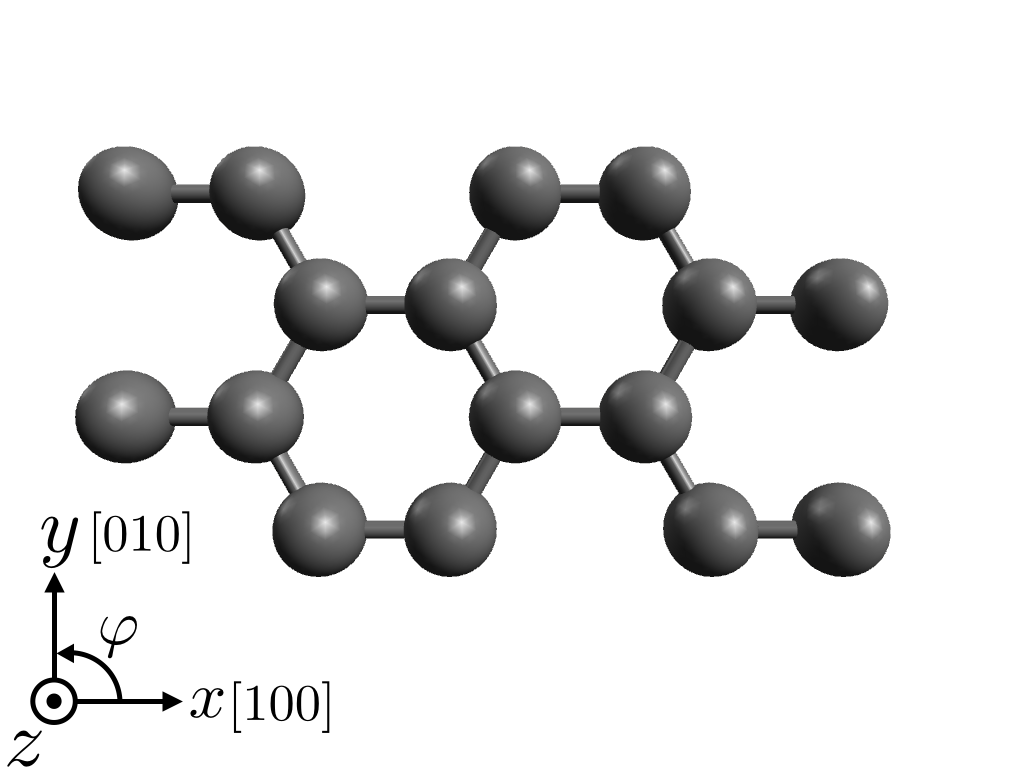
\includegraphics[width=0.49\linewidth]{figures/images/graph1}
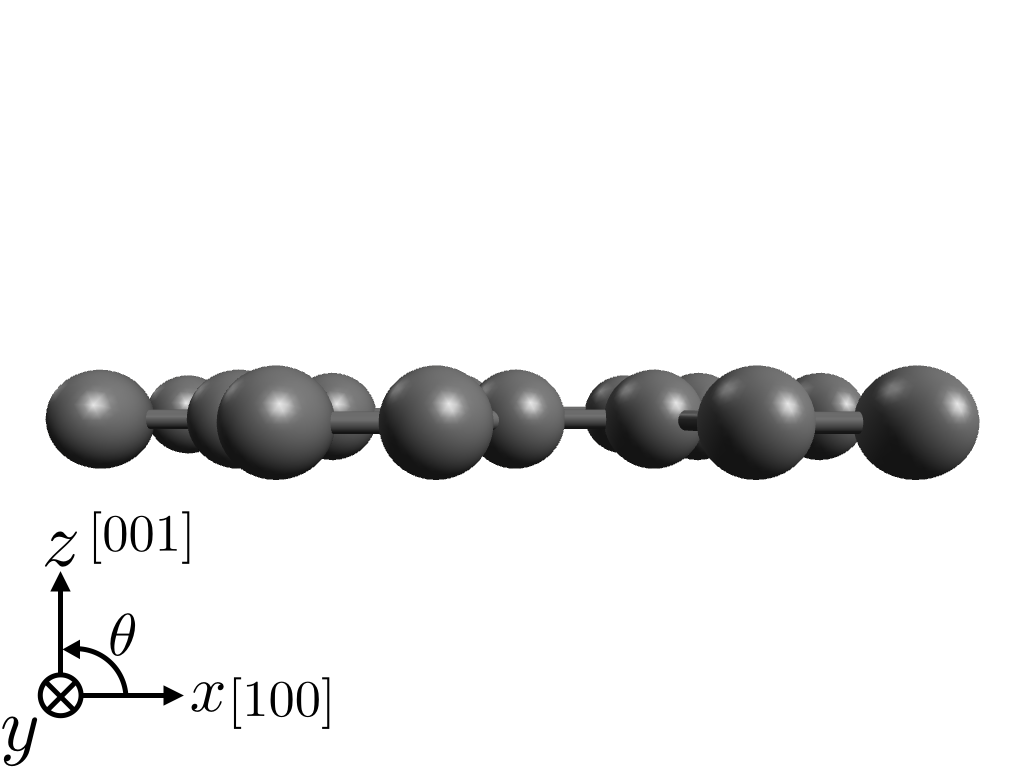
\includegraphics[width=0.49\linewidth]{figures/images/graph2}
\label{fig:graphenestrc}}
\\
\subfloat[Top and side view of C$_{16}$H$_{8}$-alt graphene structure.]
{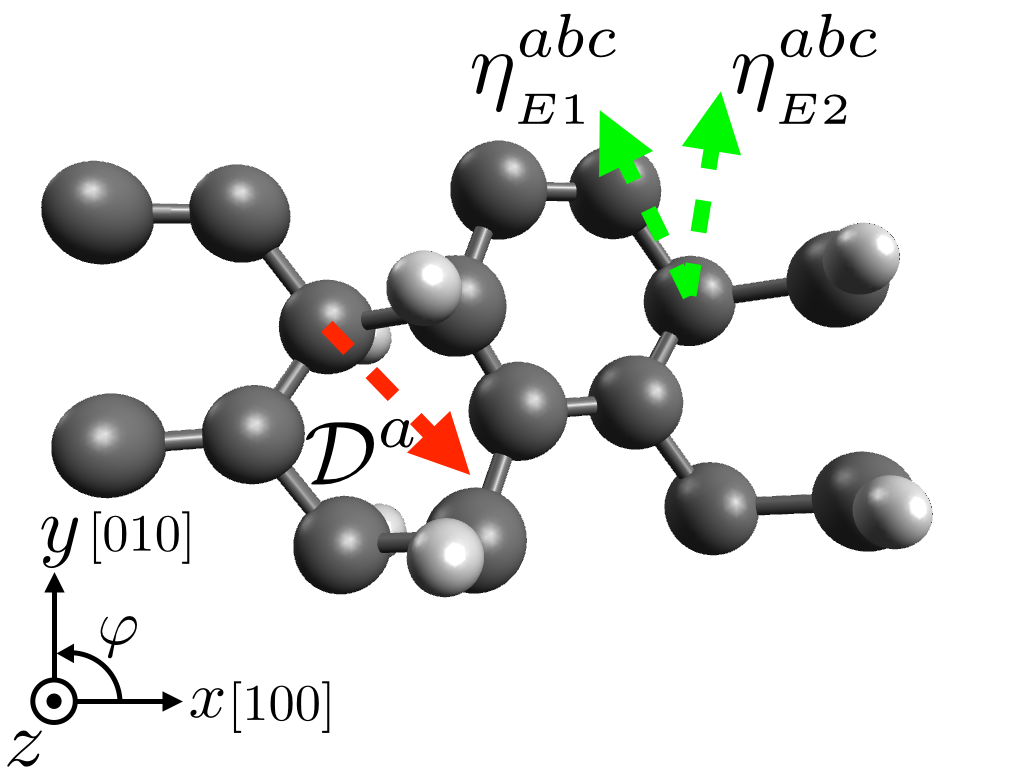
\includegraphics[width=0.49\linewidth]{figures/images/alt1}
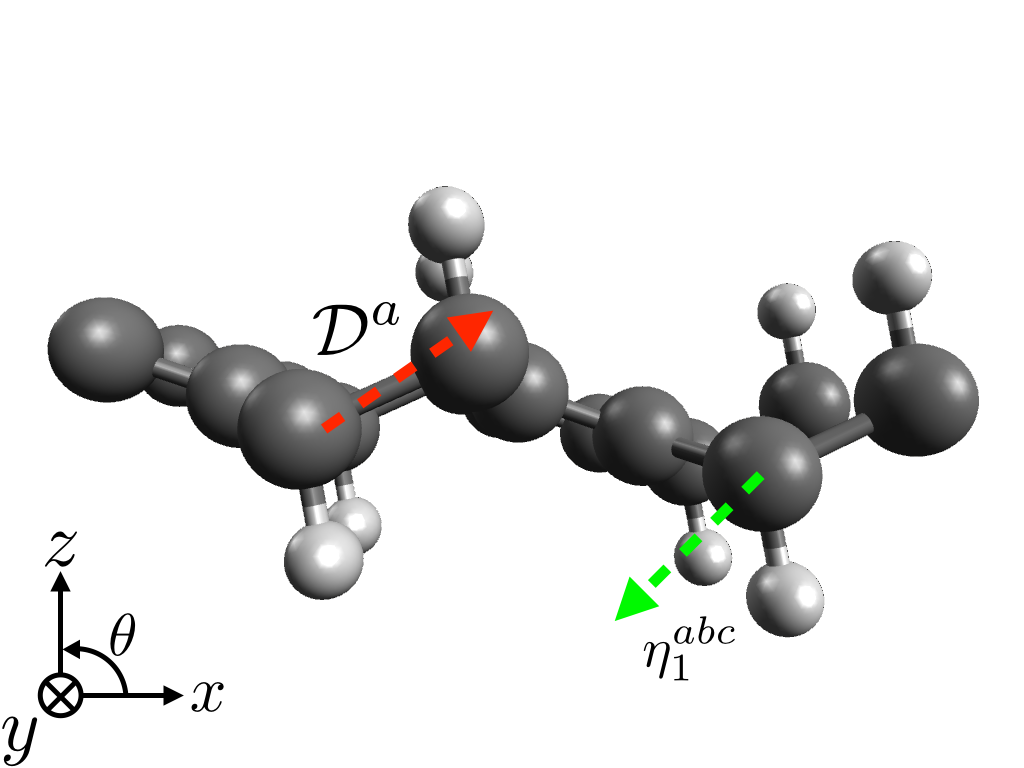
\includegraphics[width=0.49\linewidth]{figures/images/alt2}
\label{fig:altstrc}}
\\
\subfloat[Top and side view of C$_{16}$H$_{8}$-up graphene structure.]
{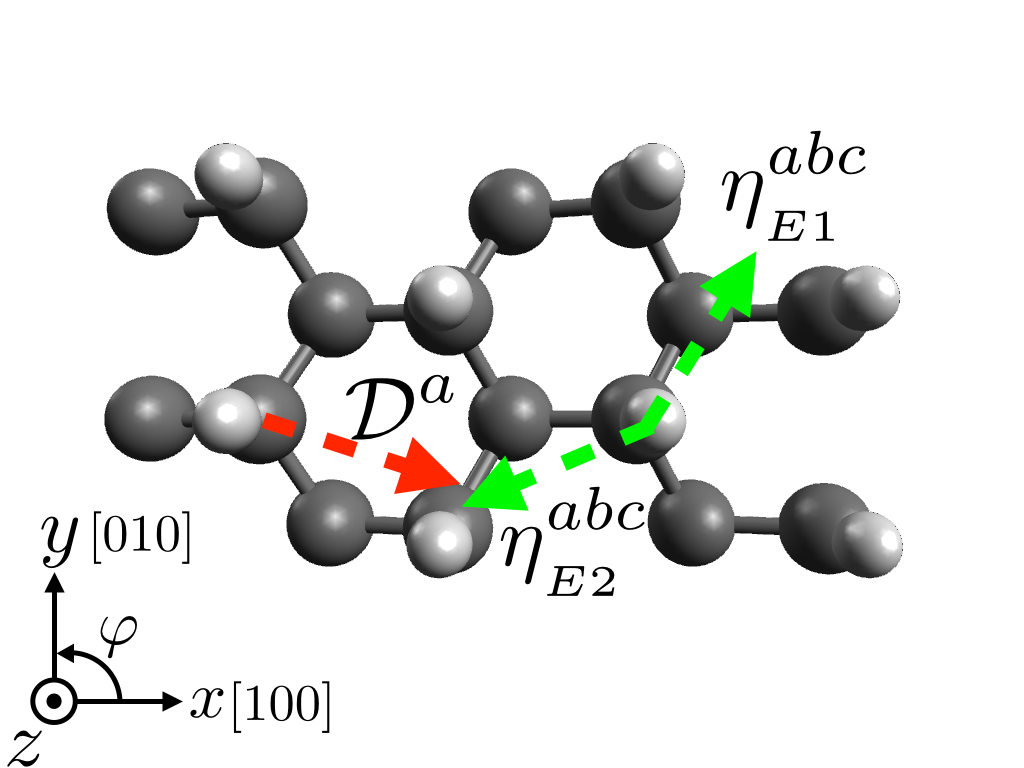
\includegraphics[width=0.49\linewidth]{figures/images/up1}
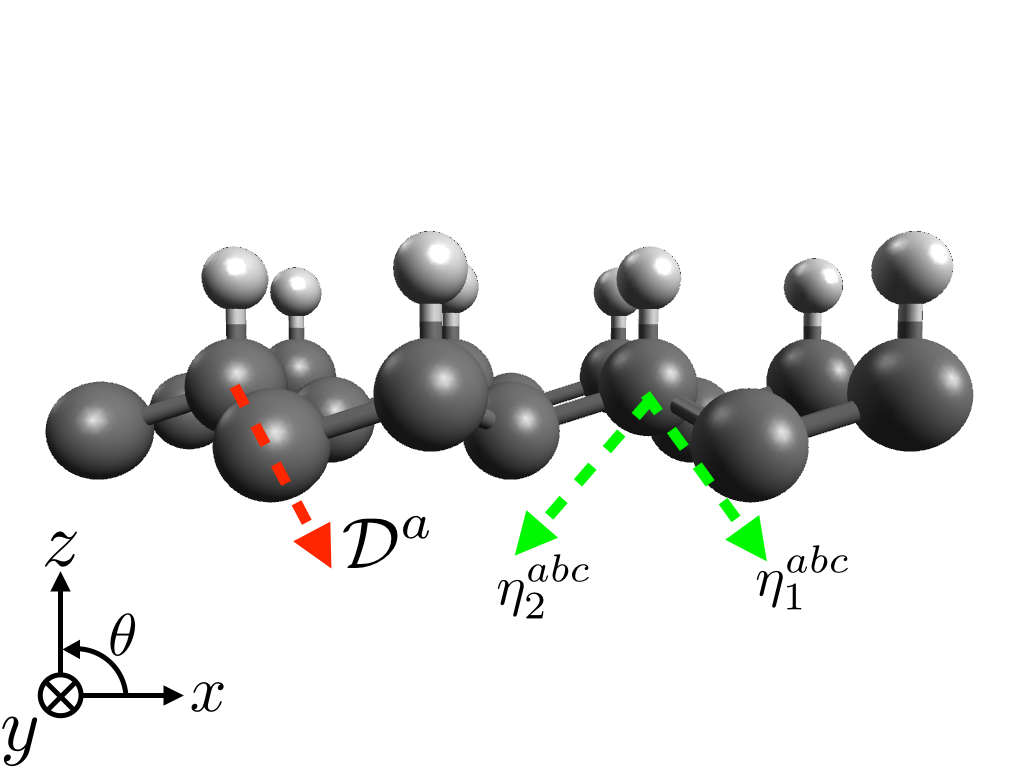
\includegraphics[width=0.49\linewidth]{figures/images/up2}
\label{fig:upstrc}}
\caption{(Color online) Diagrams of pristine graphene
(\ref{fig:graphenestrc}), and the C$_{16}$H$_{8}$-alt (\ref{fig:altstrc}), and
C$_{16}$H$_{8}$-up (\ref{fig:upstrc}) structures. The light (dark) spheres
correspond to hydrogen (carbon) atoms. We take the carbon honeycomb lattice to
be in the $xy$ plane, and the carbon-hydrogen plane to be in the $xz$ plane.
The red (green) dashed arrows in \ref{fig:altstrc} and \ref{fig:upstrc}
represent the direction where the $\mathcal{D}(\omega)$ ($\eta^{abc}(\omega)$)
point in the corresponding $xy$ and $xz$ plane. This information is explained
in subsections \ref{subsec:results-DSP} and \ref{subsec:results-eta}.
\label{fig:structures}}
\end{figure}


\subsection{Optical spin injection}

The injection and detection of spin polarized electrons into nonmagnetic
materials is the core of spintronics \cite{vzuticRMP04,fertRMP08} and an
important problem in condensed matter theory. The idea of creating and
detecting spin polarized electrons from light originates in the 1960s with
Ref. \cite{lampelPRL68}. Following that work, it was later demonstrated that
converting the angular momentum of light into electron spin is very efficient
in III-IV semiconductors \cite{dyakonovOO84}. The optical spin injection is
characterized through the dimensionless degree of spin polarization (DSP),
$\boldsymbol{\mathcal{D}}(\omega)$. The DSP quantifies the fraction of
injected electrons into the conduction bands that are spin polarized. This
effect occurs when circularly polarized light is incident on a semiconducting
material \cite{dyakonovOO84}, thus allowing electrons to move from the valence
to the conduction bands. The resulting polarization is produced by the
interaction between the electron spin and its motion caused by the spin-orbit
coupling in the material. DSP can be calculated with a full band structure
method as shown in Refs. \cite{nastosPRB07,cabellosPRB09}. There are
theoretical reports of DSPcalculations for bulk media
\cite{nastosPRB07,cabellosPRB09} and also for surfaces
\cite{mendozaPRB12,arzatePRB14}.


\subsection{Optical current injection}

The optical current injection is a second-order optical nonlinear effect that
has been the subject of research in recent years
\cite{arzatePRB14,bhatPRB05,fraserPRL99,hachePRL97,lamanAPL99}. A
photocurrent, $\mathbf{\dot{J}}(\omega)$, can be injected with a single
optical beam in noncentrosymmetric materials or at the surface of bulk
centrosymmetric materials where the symmetry inversion is broken
\cite{arzatePRB14}. This phenomenon results from the interference of one-photon 
absorption processes associated with different linear polarizations of
the light. In the process of current injection, the energy increase of the
injected carriers is provided by the electromagnetic field, meanwhile the
increase in momentum is provided by the crystal lattice \cite{arzatePRB14}.
The one-photon current injection is characterized by the current injection
tensor, $\eta^{abc}(\omega)$, and since it is generated with circularly
polarized light, this phenomenon is also called the circular photovoltaic
effect \cite{sturmanCRCP92}. This effect has been studied in bulk
semiconductors \cite{hachePRL97,sipePRB00}, two-dimensional systems
\cite{melePRB00,cabellosPRB11}, and one-dimensional nanotubes
\cite{melePRB00}. The two structures in this study, C$_{16}$H$_{8}$-alt and
C$_{16}$H$_{8}$-up, are both noncentrosymmetric and present an optical current
injection response.


\subsection{Second-harmonic generation}

Second-harmonic generation (SHG) is a nonlinear optical effect that can be
produced in noncentrosymmetric materials or at the surface of centrosymmetric
media where the inversion symmetry is broken. This phenomenon is a particular
case of sum frequency generation and is characterized through the nonlinear
susceptibility tensor, $\chi^{abc}(-2\omega;\omega,\omega)$; the resulting
nonlinear polarization in the media acts as a source for the electromagnetic
waves of frequency $2\omega$ \cite{loudonOUP00}. SHG spectroscopy techniques
bring the possibility to study material properties due to their noninvasive
and nondestructive nature, and inherent surface sensitivity. The two cases in
this study, C$_{16}$H$_{8}$-alt and C$_{16}$H$_{8}$-up, are structures with
different atomic arrangements and are noncentrosymmetric. They present SHG
from the entire structure and are efficient SHG generators. This effect has
been theoretically studied in bulk media \cite{andersonPRB15,figliozziPRL05},
two-dimensional systems \cite{mendozaPRB97,niAPL03}, and one-dimensional
nanotubes \cite{salazarPRB14,guoPRB05}.

This paper is organized as follows. In Sec. \ref{sec:theory} we present the
theory and formulas that describe the DSP, optical current injection, and SHG.
In Sec. \ref{sec:results} we describe the details of the calculations and the
corresponding spectra for the respective \emph{alt} and \emph{up} structures.
Finally, we give our conclusions in Sec. \ref{sec:conclusions}.


\section{Theory}\label{sec:theory}

In this section we report a summary of the theory for the three phenomena of
interest. For full details see Refs. \cite{nastosPRB07,mendozaPRB12} for DSP,
Refs. \cite{cabellosPRB11,sipePRB00} for optical current injection, and Ref.
\cite{andersonPRB15} for SHG. 


\subsection{Optical spin injection}\label{sec:theory-DSP}

The DSP, along a given $a$ direction is
defined as
$\mathcal{D}^{a}(\omega)=\dot{S}^{a}(\omega)/(\hbar/2)\dot{n}(\omega)$
\cite{mendozaPRB12}. The spin generation rate, $\dot{S}^{a}(\omega)$, and the
carrier generation rate, $\dot{n}(\omega)$, are given by
\begin{align}
\dot{S}^{a}(\omega)&= 
\zeta^{abc}(\omega)E^{b}(-\omega)E^{c}(\omega), \label{eq:spinrate} \\
\dot{n}(\omega)&= 
\xi^{ab}E^{a}(-\omega)E^{b}(\omega), \label{eq:carrierrate}
\end{align}
where $\zeta^{abc}(\omega)$ are the spin injection rate tensor components and
$\xi^{bc}(\omega)$ are the carrier generation rate tensor components
\cite{arzatePRB14}. The superscripts denote Cartesian directions and if repeated
are to be summed over. Then, assuming an incoming circularly polarized beam at
normal incidence that propagates along the $-z$ direction, $\mathbf{E}(\omega) =
E_{0}(\omega)(\mathbf{\hat{x}} - i\mathbf{\hat{y}})/\sqrt{2}$, with $E_{0}$ as
the intensity, we obtain $\mathcal{D}^{a}(\omega)$ from Eqs.
\eqref{eq:spinrate} and \eqref{eq:carrierrate} \cite{arzatePRB14} as
\begin{equation}\label{eq:D^i}
\mathcal{D}^{a}(\omega) =  
\frac{-4i\zeta^{axy}(\omega)}
    {\hbar\left(\xi^{xx}(\omega) + \xi^{yy}(\omega)\right)}.
\end{equation}
It is possible to generate current injection along all three orthogonal
Cartesian directions with an incident circularly polarized beam and so the
absolute DSP can be obtained \cite{arzatePRB14} by 
\begin{equation}\label{eq:dsptotal}
\mathcal{D}(\omega) =
\sqrt{(\mathcal{D}^{x}(\omega))^{2} + 
      (\mathcal{D}^{y}(\omega))^{2} +
      (\mathcal{D}^{z}(\omega))^{2}
      }.
\end{equation}


\subsection{Optical current injection}\label{sec:theory-OCI}

The optical current injection is given \cite{arzatePRB14} by
\begin{equation*}
\mathbf{\dot{J}}^{a}_{\text{inj}}(\omega) =
\eta^{abc}(\omega)E_{b}(\omega)E_{c}(\omega), \label{eq:current}
\end{equation*}
where $\eta^{abc}(\omega)$ is the current injection tensor which quantifies
the current injection along the $a$ direction that is optically injected. To
maximize $\mathbf{\dot{J}}^{a}_{\text{inj}}(\omega)$ we use a circularly
polarized beam at normal incidence in the $-z$  direction, $\mathbf{E}(\omega)
= E_{0}(\omega)(\mathbf{\hat{x}} - i\mathbf{\hat{y}})/\sqrt{2}$. For a layered
system we have that the total contribution to $
\eta^{abc}(\omega)$ is given \cite{arzatePRB14} by
\begin{equation}\label{eq:eta}
\eta^{abc}(\omega)=
\ell_{\mathrm{eff}}\sum_{\ell=1}^{N_{\mathrm{eff}}}\eta^{abc}(\ell|\omega)
\end{equation}
where $\eta^{abc}(\ell|\omega)$ gives the contribution from the corresponding
$\ell^{\mathrm{th}}$ layer to the total injection current tensor. For our structures
the sum in Eq. \eqref{eq:eta} is carried out from the top layer, $\ell=1$, to
the last layer that have contributions to the total response, being the third layer
for the \emph{alt} structure and second layer for the \emph{up} structure. Like in
optical spin injection, it is possible to generate current injection along all
three directions with an incident circularly polarized beam. Analogously to Eq.
\eqref{eq:dsptotal} it is possible to have the absolute $\eta(\omega)$
\cite{arzatePRB14} as
\begin{equation}\label{eq:etatotal}
\eta(\omega) =
\sqrt{(\eta^{xxy}(\omega))^{2} +
      (\eta^{yxy}(\omega))^{2} +
      (\eta^{zxy}(\omega))^{2}
      }.
\end{equation}


\subsection{Second-harmonic generation}\label{sec:theory-SHG}
The second-order nonlinear polarization is given \cite{andersonPRB15} by
\begin{equation*}\label{eq:pol}
\mathcal{P}(2\omega) = 
\chi^{abc}(-2\omega;\omega,\omega)E^{b}(\omega)E^{c}(\omega)
\end{equation*} where $\chi^{abc}(-2\omega;\omega,\omega)$ is the nonlinear
susceptibility tensor responsible for the SHG, where we follow Ref.
\cite{andersonPRB15} to calculate it. The 
formalism of Ref. \cite{andersonPRB15} includes (i) the scissors correction,
(ii) the contribution of the nonlocal part of the pseudopotentials, and (iii)
the cut function used to select the individual contribution for a given layer.
Analogously to the case of optical current injection we have that for a layered
system the total contribution for the second-order susceptibility tensor can be
obtained by
\begin{equation}
\boldsymbol{\chi}^{\mathrm{abs}}(-2\omega;\omega,\omega) = 
\sum_{\{\ell\}} \boldsymbol{\chi}^{\mathrm{abs}}_{\ell}(-2\omega;\omega,\omega)
\end{equation}
where $\ell$ denote a particular layer chosen.


\section{Results}\label{sec:results}

We present the results for {$D^{a}(\omega)$}, {$\eta^{abc}(\omega)$}, and
$\chi^{abc}(-2\omega;\omega,\omega)$ for the C$_{16}$H$_{8}$-alt and
C$_{16}$H$_{8}$-up structures. As mentioned before, both cases are 
semi-infinite carbon systems with 50\% of hydrogenation in two different
arrangements. The \emph{alt} system has alternating hydrogen atoms on the
upper and bottom sides of the carbon sheet, while the \emph{up} system has H
only on the upper side. Both structures are noncentrosymmetric and have a
thickness of 2.944\,{\AA} and 2.766\,{\AA}, respectively. The coordinates for
the \emph{alt} and \emph{up} unit cells of the structures are presented in
Tables \ref{tab:altstrc} and \ref{tab:upstrc} with the corresponding layer
divisions. We take the carbon honeycomb lattice to be in the $xy$ plane for
both structures and the carbon-hydrogen bonds in the perpendicular $xz$ plane
as depicted in Fig.\ref{fig:structures}. In order to represent the directions
where the absolute values of the $\mathcal{D}(\omega)$ and $\eta(\omega)$
(Eqns. \eqref{eq:dsptotal} and \eqref{eq:etatotal}) we define the azimuthal
angle $\varphi$ in the $xy$ plane and the polar angle $\theta$ in the $xz$
plane both measured positive in the counterclockwise starting from $x$, as
usual in the polar coordinate system, as shown in Fig. \ref{fig:structures}.

\begin{table}[t]
% \sidecaption
\centering
\begin{tabular}{cccc}
\hline
\hline
Atom type &  \multicolumn{3}{c}{Position [\AA] } \\
\cline{2-4}
& $x$ & $y$ & $z$ \\
\hline
\multicolumn{2}{l}{First layer}\\
H & 2.46067 & 0.34243 & 13.74110 \\
\multicolumn{2}{l}{Second layer}\\
C & 2.46067 & 0.03082 & 12.66504 \\
C & 3.69101 & 3.49684 & 12.42680 \\
C & 3.69101 & 2.18585 & 12.11058 \\
C & 2.46067 & 1.38987 & 11.87240 \\
\multicolumn{2}{l}{Third layer}\\
H & 2.46067 & 1.07817 & 10.79635 \\
\hline
\hline
\end{tabular}
\caption[]{%
Atom types and positions for the C$_{16}$H$_{8}$-alt structure unit cell in
Cartesian coordinates. The system was separated into three layers: (i) top
hydrogen atoms, (ii) central carbon atoms, and (iii) bottom hydrogen atoms.
\label{tab:altstrc}}
\end{table}
\begin{table}[t]
% \sidecaption
\centering
\begin{tabular}{cccc}
\hline
\hline
Atom type &  \multicolumn{3}{c}{Position [\AA]} \\
\cline{2-4}
& $x$ & $y$ & $z$ \\
\hline
\multicolumn{2}{l}{First layer}\\
H &  -0.00000 & 0.00129 & 25.71942 \\
H & \ 2.32500 & 4.02509 & 25.71904 \\
\multicolumn{2}{l}{Second layer}\\
C & \ 2.32497 & 4.02980 & 23.40860 \\
C &  -0.00000 & 0.00415 & 23.40763 \\
C &  -0.00000 & 2.68121 & 22.96963 \\
C & \ 2.32500 & 6.70665 & 22.95301 \\
\hline
\hline
\end{tabular}
\caption[]{%
Atom types and positions for the C$_{16}$H$_{8}$-up structure unit cell in
Cartesian coordinates. The system was separated in two layers: (i) top
hydrogen atoms and (ii) bottom carbon atoms.}
\label{tab:upstrc}
\end{table}

We used the ABINIT code \cite{gonzeCPC09} for the calculation of the 
self-consistent ground state and the Kohn-Sham states using density functional
theory in the local density approximation (DFT-LDA) with a planewave basis. We
used Hartwigsen-Goedecker-Hutter (HGH) relativistic separable dual-space
Gaussian pseudopotentials \cite{hartwigsenPRB98} that include spin-orbit
interaction for calculating $D^{a}(\omega)$. For the calculations of
{$\eta^{abc}(\omega)$} and $\chi^{abc}(-2\omega;\omega,\omega)$ we used
Troullier-Martins pseudopotentials \cite{troullierPRB91} that are fully
separable nonlocal pseudopotentials in the Kleiman-Bylander form
\cite{kleinmanPRL82}. These are required for calculating the contribution from
the nonlocal part of the pseudopotentials in the SHG response and this
calculation is carried out using the DP code \cite{olevanoDP}. For convergence
of our results we used a cutoff energies of 65\,Ha and 40\,Ha and the energy
eigenvalues and matrix elements were calculated using 14452 \textbf{k} points
and 8452 \textbf{k} points in the irreducible Brillouin zone (IBZ) for the
\emph{alt} and \emph{up} cases, respectively. Also, the \emph{alt} and
\emph{up} structures present LDA energy band gap of  0.72\,eV and 0.08\,eV,
respectively.
\textcolor{red}{
We note that within DFT, the LDA is but one of many possible methods that can
be used to calculate the electronic structure of materials. Recent studies on
graphene \cite{karamanisJPCC15,botelloACR14} present some of the differences
in calculated values from several of these methods. We note that the LDA is on
par with these other approaches. It is also well known that all DFT methods
predict a band gap for the material that differs from experiment. This can be
corrected by using other \emph{ab initio} techniques such as the GW
approximation \cite{onidaRMP02}, but this technique is computationally very
expensive and is outside the scope of this paper. Nevertheless, DFT still
remains a mainstream tool for calculating diverse properties derived from the
electronic band structure. }

Our systems under study where divided in layers, this has been done to analyze
the contribution of each layer for the $\eta^{abc}(\omega)$ and
$\chi^{abc}(-2\omega;\omega,\omega)$ responses. The
\emph{alt} system is divided into three layers comprised of the top H atoms,
the carbon plane, and the bottom H atoms. The \emph{up} system is divided into
two layers comprised of the top H atoms and the carbon plane. The layer
selections for the unit cells are shown explicitly in Tables \ref{tab:altstrc}
and \ref{tab:upstrc}.


\subsection{Optical spin injection}\label{subsec:results-DSP}

In Fig. \ref{fig:Da} we show the $D^{a}(\omega)$ spectra for the
C$_{16}$H$_{8}$-alt and C$_{16}$H$_{8}$-up systems resulting from the
evaluation of the Eq. \eqref{eq:D^i}. Values over (under) zero define a
positive (negative) direction of spin polarization along the \emph{a}
direction with respect the three Cartesian vectors shown in Fig.
\ref{fig:structures}. For both cases, the onset of the response is when the
energy of the incoming light is the same as the gap energy. The \emph{alt}
system presents nearly 40\% $\mathcal{D}^{a}(\omega)$ in the $x$ and $y$
directions and after 0.72\,eV the DSP rapidly vanishes. Using Eq.
\eqref{eq:dsptotal} we have that the \emph{alt} system presents an absolute
magnitude $\mathcal{D}(\omega)$ = 61\% for a frequency of 0.72\,eV with
$\varphi = -46^{\circ}$ and $\theta=35^{\circ}$. In Fig. \ref{fig:altstrc} the
dashed red arrow depicts how $\mathcal{D}(\omega)$ is oriented in the $xy$ and
$xz$ planes at the angles mentioned above. For the
\emph{up} structure we have nearly 60\% DSP in the $z$ direction. Using Eq.
\eqref{eq:dsptotal} we have that the \emph{up} structure presents an absolute
magnitude $\mathcal{D}(\omega)$ = 64\% for a frequency of 0.08\,eV,
with$\varphi = -18^{\circ}$ and $\theta = -62^{\circ}$. In Fig.
\ref{fig:upstrc} the dashed red arrow depicts how $\mathcal{D}(\omega)$ is
oriented in the $xy$ and $xz$ planes at the angles mentioned above.

In Table \ref{tab:dacomp} we present a comparison of the absolute maximum
values of $\mathcal{D}^{a}(\omega)$ in a given direction for different
materials and the corresponding direction and energy at which they are
reached. From this table we have that the \emph{alt} and \emph{up} systems
have less DSP than the Si(111)-As $1\times1$ and the bulk CdSe cases, but are
comparable to the Si(111)-In $8\times2$, bulk Si, and bulk GaAs systems.
Si(111)-In $8\times2$ and \emph{alt} both have maxima around 0.72\,eV, which
is in the near infrared range. Conversely, the maxima for Si(111)-As
$1\times1$, bulk Si, and bulk GaAs all occur in the optical energy range.
\begin{table}[b]
\centering
\sidecaption
\begin{tabular}{lcccc}
\hline
\hline
Case & Energy &  \multicolumn{2}{c}{$D^{a}$} &  Ref.\\
\cline{3-4}   & [eV]   & direction & [\%] \\
\hline
C$_{16}$H$_{8}$-alt    & 0.72 & y & 39  & * \\
C$_{16}$H$_{8}$-up     & 0.08 & z & 57  & * \\
Si(111)-In $8\times2$  & 0.74 & z & 32  & \cite{arzatePRB14}\\
Si(111)-As $1\times1$  & 2.20 & z & 100 & \cite{mendozaPRB12}\\
Bulk Si                & 3.44 & z & 30  & \cite{nastosPRB07}\\
Bulk GaAs              & 1.50 & z & 50  & \cite{nastosPRB07,bhatPRB05}\\
Bulk CdSe              & 1.80 & z & 100 & \cite{nastosPRB07}\\
\hline
\hline
\end{tabular}
\caption[]{Comparison of the reported absolute maximum values of {$D^{a}$} for
different materials. ($^{*}$This work)}
\label{tab:dacomp}
\end{table}

\begin{figure}[t]
\subfloat{\includegraphics[width=\linewidth]{figures/dsp-alt}}
\hfill
\subfloat{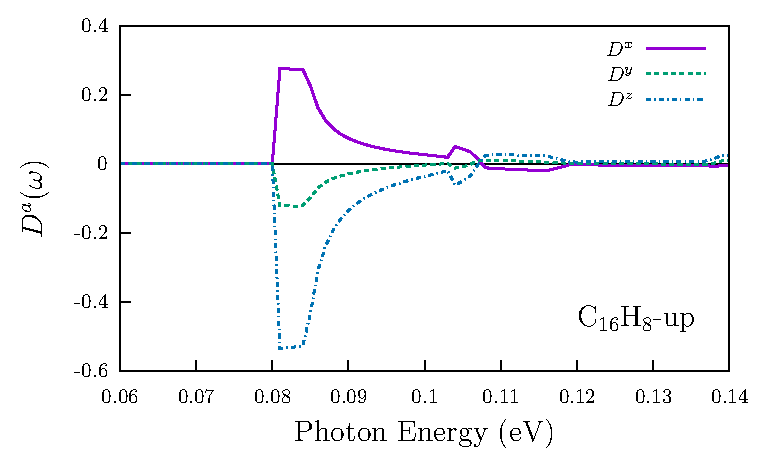
\includegraphics[width=\linewidth]{figures/dsp-up}}
\caption{(Color online) Spectra of the degree of spin polarization
{$D^{a}(\omega)$}, for the C$_{16}$H$_{8}$-alt and
C$_{16}$H$_{8}$-up.\label{fig:Da}}
\end{figure}


\subsection{Optical current injection}\label{subsec:results-eta}

In Fig. \ref{fig:alt-eta} we present the three components for the total
$\eta^{abc}(\omega)$ for the 
\emph{alt} structure along with the layer by layer analysis in which we split
the total response spectra in the corresponding contributions of each layer
mentioned above. We establish two energy values of interest for each structure
where there are large values for the response in the spectra. For the
\emph{alt} structure we choose $\omega_{1} = 0.97\,\mathrm{eV}$ and $\omega_{2} =
1.31\,\mathrm{eV}$. For the layer by layer analysis corresponding to the
contributions of each atomic layer to the total response, we note that all
three layers contribute toward $\eta^{xxy}(\omega_{1})$ with the carbon
and top H layers providing the principal contributions. For $\eta^{xxy}(\omega_{2})$, the
dominating layers are the carbon and bottom H layers with minimal contribution
from the top H layer. For $\eta^{yxy}(\omega_{1})$ component is also
formed by contributions from all three layers but dominated by the sum of the
top and bottom H layers. The carbon layer response is negative at that point,
and cancel the response from the other two layers. For
$\eta^{yxy}(\omega_{2})$ the spectrum is completely dominated by the bottom H layer, with
almost no contribution from the others. Lastly 
$\eta^{zxy}(\omega_{1})$ component is entirely produced from the carbon layer,
since the H layers provide no response whatsoever. This component is negligible
at $\omega_{2}$ and note that the response for all three components vanishes after
1.75\,eV. Using Eq. \eqref{eq:etatotal}, we find that the absolute current
injection $\eta(\omega_{1})$ is
$5.10\,\mathrm{mC}^{3}/\mathrm{J}^{2}\mathrm{s}^{2}$ with angles
$\varphi=116^{\circ}$ and $\theta=-172^{\circ}$. For the second value of energy we find that
$\eta(\omega_{2})=2.32\,\mathrm{mC}^{3}/\mathrm{J}^{2}\mathrm{s}^{2}$ with angles
$\varphi=81^{\circ}$ and $\theta=12^{\circ}$. In Fig.
\ref{fig:altstrc}, the green dashed arrows represent the directions for
$\eta(\omega_{1})$ and $\eta(\omega_{2})$. As mentioned
previously, $\varphi$ is located in the $xy$ plane, and $\theta$ is located in
the $xz$ plane.

\begin{figure}[t]
\centering
\subfloat{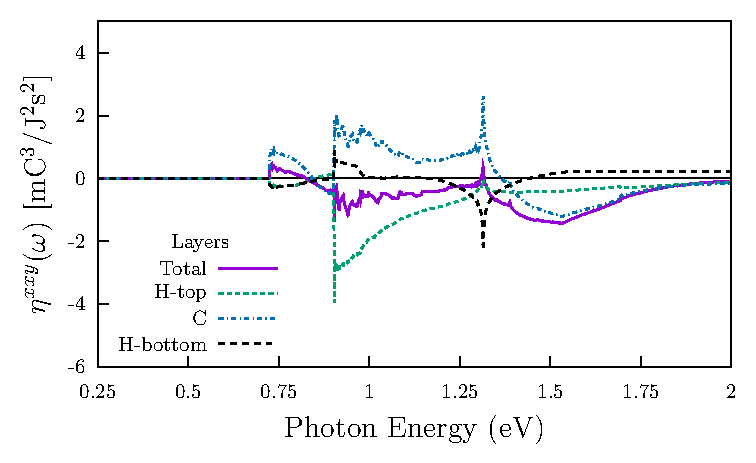
\includegraphics[width=\linewidth]{figures/eta-alt_x}}\\
\subfloat{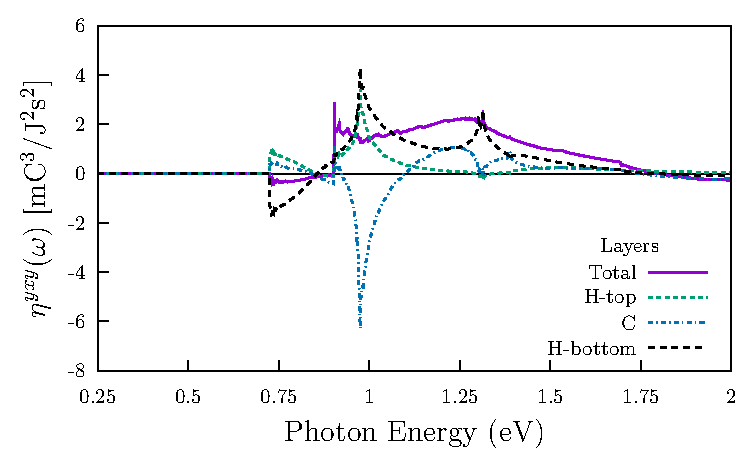
\includegraphics[width=\linewidth]{figures/eta-alt_y}}\\
\subfloat{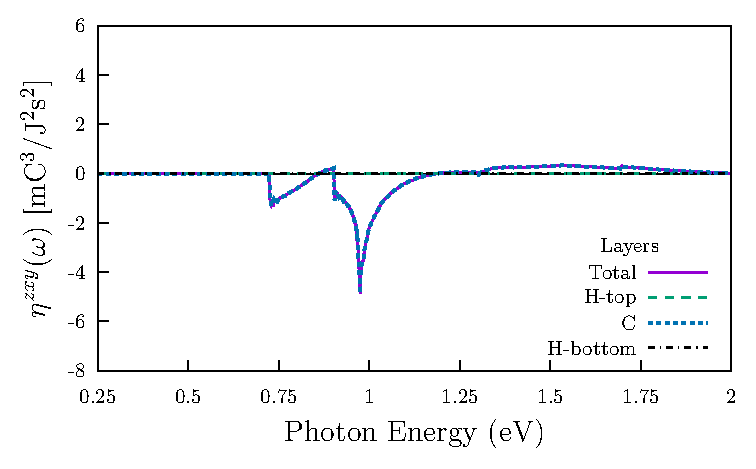
\includegraphics[width=\linewidth]{figures/eta-alt_z}}
% 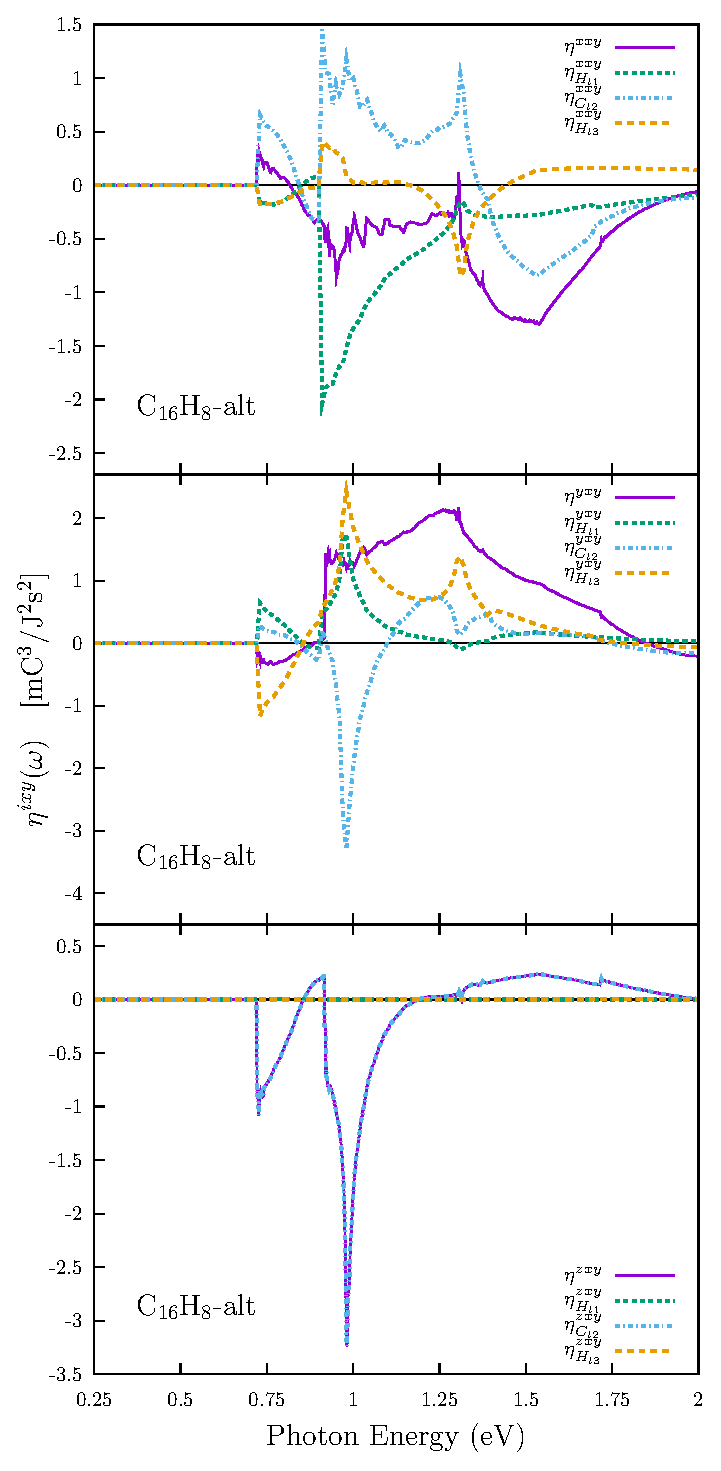
\includegraphics[width=\linewidth]{alt/alt-eta-layers}
\caption{(Color online) Spectra of the current injection tensor
{$\eta^{abc}(\omega)$} for C$_{16}$H$_{8}$-alt. Solid lines are the total
current injection and dashed lines correspond to the layer
contributions.\label{fig:alt-eta}}
\end{figure}

\begin{figure}[b]
\centering
\subfloat{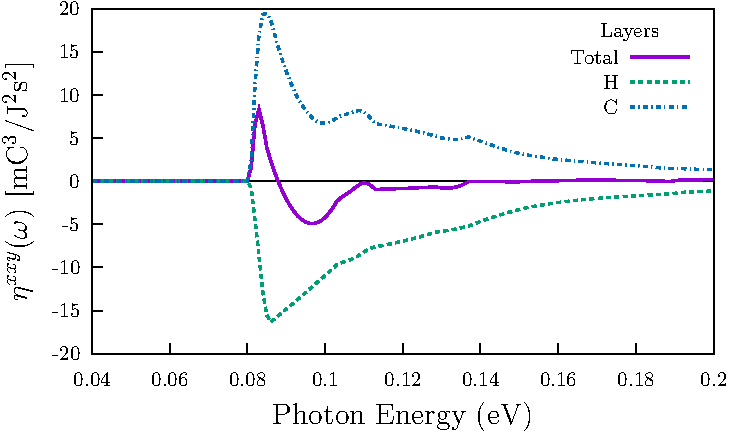
\includegraphics[width=\linewidth]{figures/eta-up_x}}\\
\subfloat{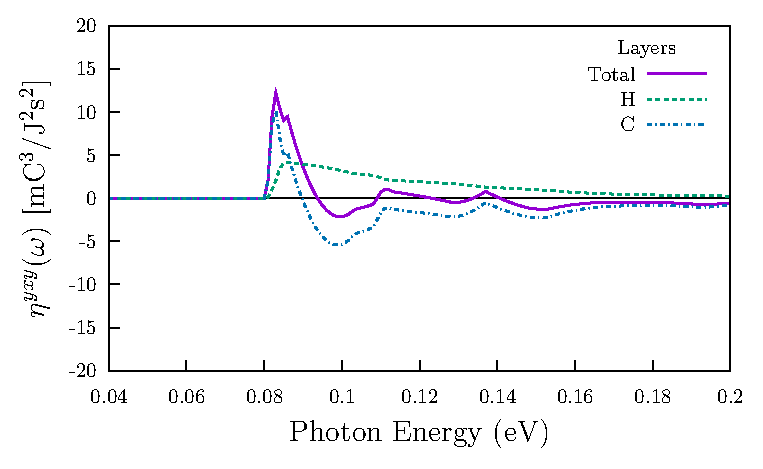
\includegraphics[width=\linewidth]{figures/eta-up_y}}\\
\subfloat{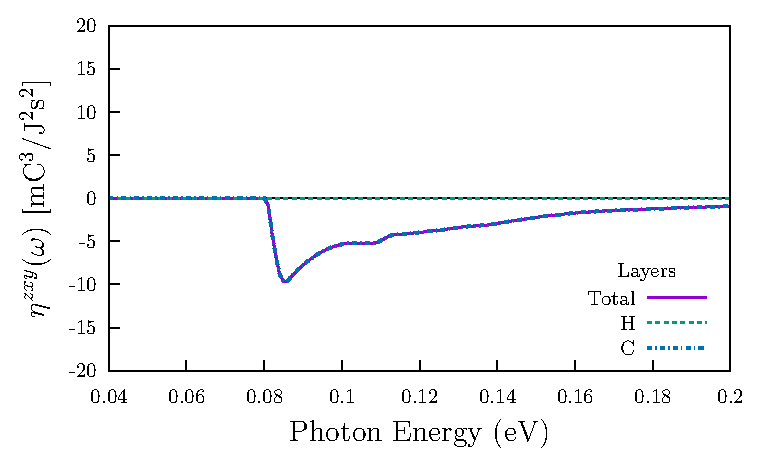
\includegraphics[width=\linewidth]{figures/eta-up_z}}
% 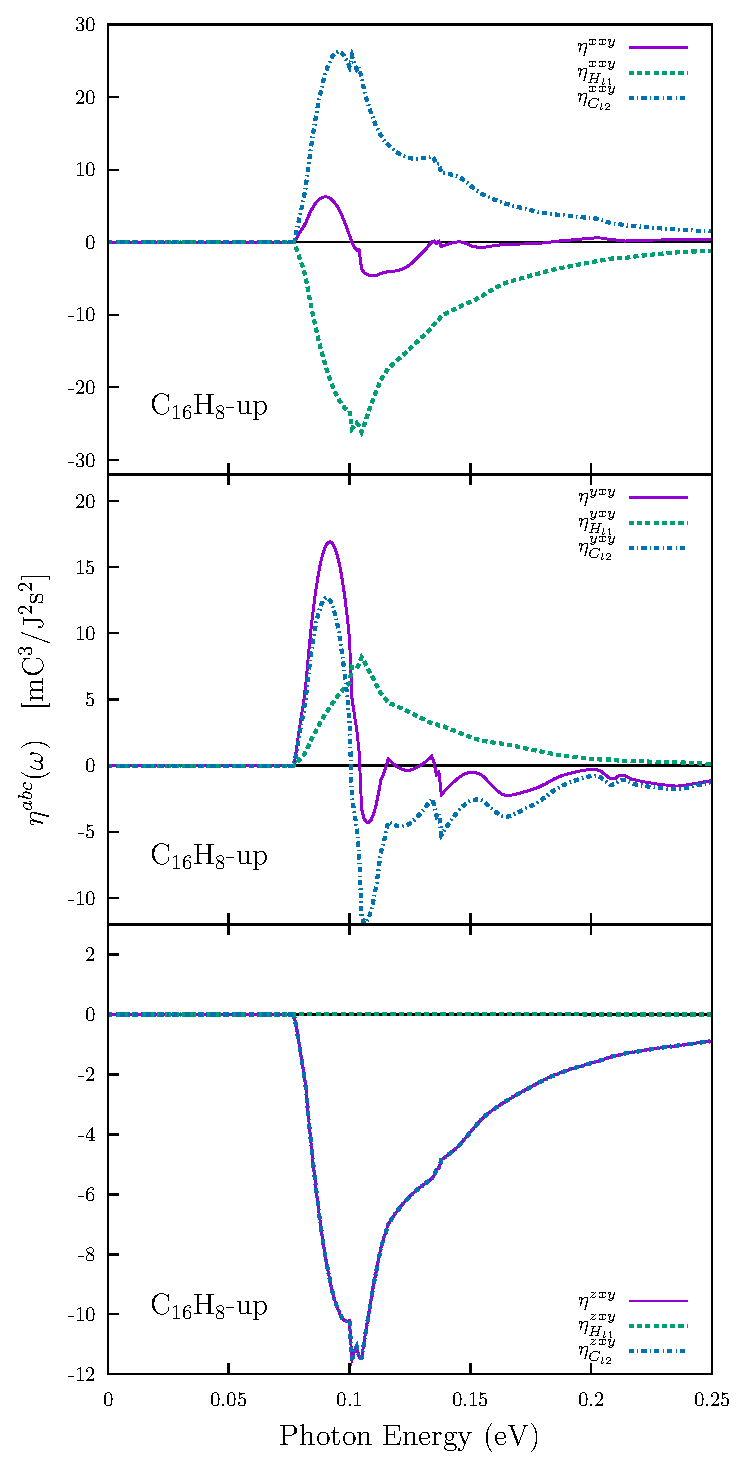
\includegraphics[width=\linewidth]{up/up-eta-multiplot}
\caption{(Color online) Spectra of the current injection tensor
{$\eta^{abc}(\omega)$} for C$_{16}$H$_{8}$-up. Solid lines are the total
current injection and dashed lines correspond to the layer
contributions.\label{fig:up-eta}}
\end{figure}


Analogously, Fig. \ref{fig:up-eta} presents the three components of the total
$\eta^{abc}(\omega)$ for the \emph{up} structure including the layer by layer
spectra. We also establish two energy values of interest for this structure,
choosing $\omega_{1} = 0.09\,\mathrm{eV}$ and $\omega_{2} = 0.10\,\mathrm{eV}$. For
$\eta^{axy}(\omega_{1})$, the carbon layer dominates the total response for all three
components. For $\eta^{yxy}(\omega_{2})$ and $\eta^{zxy}(\omega_{2})$ the carbon layer
dominates the response of the system, but both the H and carbon layer contribute
significantly to $\eta^{xxy}(\omega_{2})$. Identically to the \emph{alt} structure,
the $\eta^{zxy}(\omega)$ component presents no response from the H layer.  We
note that the response for all three components vanishes after 0.2\,eV. Using
Eq. \eqref{eq:etatotal}, we find that the absolute current injection $\eta(\omega_{1})$
is $15.12\,\mathrm{mC}^{3}/\mathrm{J}^{2}\mathrm{s}^{2}$ with angles
$\varphi=58^{\circ}$ and $\theta=-54^{\circ}$. Also, we find that
$\eta(\omega_{2})=7.62\,\mathrm{mC}^{3}/\mathrm{J}^{2}\mathrm{s}^{2}$ with angles
$\varphi=-157^{\circ}$ and $\theta=-131^{\circ}$. As before, we present the
directions for $\eta(\omega)$ in Fig. \ref{fig:upstrc} using green dashed
arrows.

In Table \ref{tab:etacomp} we present a comparison of the maximum values of
different components of $\eta^{abc}(\omega)$ reported for different materials
and the corresponding energy at which they are achieved. Excluding bulk CdSe,
the \emph{alt} and \emph{up} structures have larger values for the current
injection tensor than the other materials. The Si(111)-In $8\times 2$ surface
has peak values close to 1.25\,eV, that is similar to the \emph{alt} structure.
However, the latter has more than six times the value of $\eta^{yxy}(\omega)$.

\begin{table}%
\centering
\sidecaption
\begin{tabular}{lcccc}
\hline
\hline
Structure & Energy &  \multicolumn{2}{c}{$\eta^{abc}(\omega)$} &  Ref.\\
\cline{3-4}
          & [eV]   & $abc$ & [mC$^{3}$/J$^{2}$s$^{2}$] \\
\hline
C$_{16}$H$_{8}$-alt     & 0.97  & zxy & 4.86  & *     \\
C$_{16}$H$_{8}$-up      & 0.09  & yxy & 12.22 & *     \\
Si(111)-In $8\times2$   & 1.24  & yxy & 0.35  & \cite{arzatePRB14}  \\
Si(111) $2\times1$      & 0.75  & yxy & 1.22  & \cite{cabellosPRB11} \\
GaAs(110) clean         & 4.30  & yxy & 0.30  & \cite{cabellosPRB11}     \\
GaS (110)-Sb            & 4.60  & yxy & 0.17  & \cite{cabellosPRB11}\\
Bulk CdSe               & 1.80  & yyz & 90.0$^{\star}$  & \cite{lamanAPL99}\\
\hline
\hline
\end{tabular}
\caption[]{%
Comparison of the highest reported absolute values of {$\eta^{abc}(\omega)$}
for different structures. ($^{*}$This work. $^{\star}$Experimental value.)}
\label{tab:etacomp}
\end{table}


\subsection{Second-harmonic generation}

Both the \emph{alt} and \emph{up} structures are triclinic class 1 systems
where all 27 components of $\chi^{abc}(-2\omega;\omega,\omega)$ are nonzero,
with 18 independent components \cite{popovbook}. In Figs. 
\ref{fig:shg-high-alt} and \ref{fig:shg-high-up} we present the absolute value
of the three largest components for each structure. For the \emph{alt} system,
we note that all components present two peaks around 0.5\,eV and 1.0\,eV. The
first peak is completely produced by $2\omega$ resonances, while the second
peak is produced by a mixture of both $1\omega$ and $2\omega$ resonances, with
the latter dominating for all components. The \emph{up} structure  has one
predominant peak around 0.04\,eV that is completely produced by $2\omega$
transitions. All components have an additional feature close to 0.09\,eV
dominated by $1\omega$ transitions.

Figs. \ref{fig:shg-lay-alt} and \ref{fig:shg-lay-up} present a layer by layer
analysis for the largest component of $|\chi^{abc}(-2\omega;\omega,\omega)|$
for each structure. For the \emph{alt} structure, the first feature of
$|\chi^{xyy}(-2\omega;\omega,\omega)|$ is generated by contributions from all
three layers while the second feature is dominated by the carbon layer. For the
\emph{up} structure, $|\chi^{yxx}(-2\omega;\omega,\omega)|$ is completely
dominated by the carbon plane with almost no response from the H layer.
Additionally, we note that both structures are very efficient at SHG, with
$\chi^{abc}(-2\omega;\omega,\omega)$ values in the thousands of pm/V for
\emph{alt} and millions of pm/V for \emph{up}. The \emph{up} structure, with
only the H and carbon layers, has a high degree of noncentrosymmetry and is
therefore an excellent candidate for SHG. In table \ref{tab:shgcomp} we show a
comparison of the maximum response reported for different structures.


\begin{figure}[t]
\subfloat[The three largest components of 
$|\chi^{abc}(-2\omega;\omega,\omega)|$ for the \emph{alt} structure.
\label{fig:shg-high-alt}]
{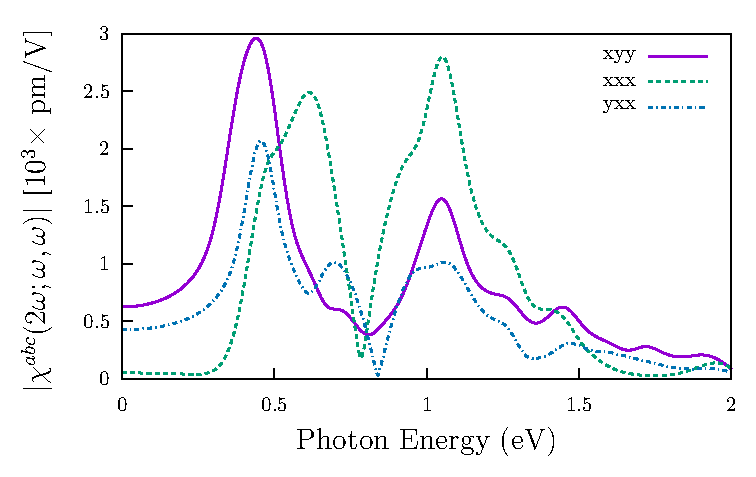
\includegraphics[width=\linewidth]{figures/shg-vnl-alt}}\\
\subfloat[Layer by layer spectra for $|\chi^{xyy}(-2\omega;\omega,\omega)|$ 
for the \emph{alt} structure.
\label{fig:shg-lay-alt}]
{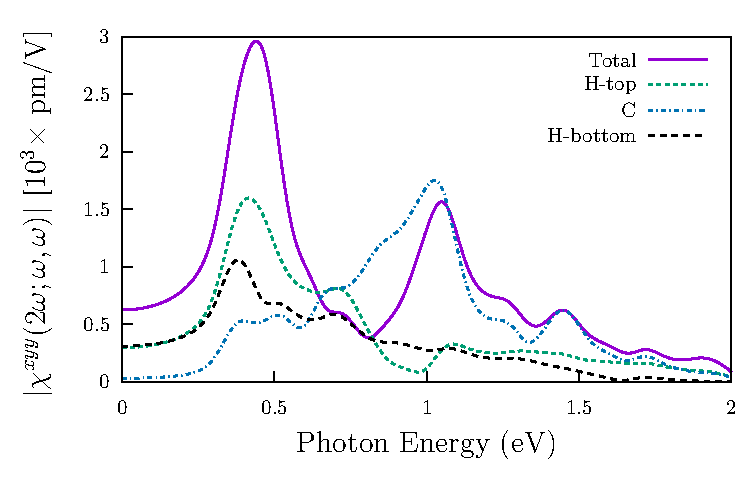
\includegraphics[width=\linewidth]{figures/shg-lay-alt}}
\caption{(Color online) SHG spectra for the \emph{alt} structure.
\label{fig:shg-vnl-alt}}
\end{figure}


\begin{figure}[t]

\subfloat[The three highest values of $|\chi^{abc}(-2\omega;\omega,\omega)|$ 
for the \emph{up} structure. \label{fig:shg-high-up}]
{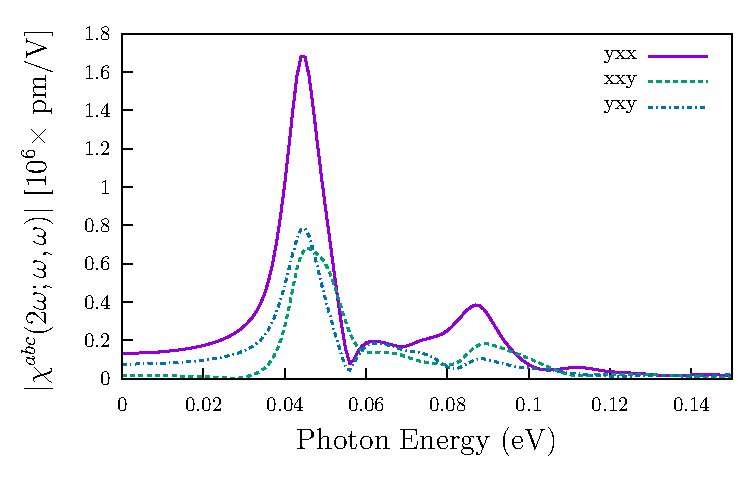
\includegraphics[width=\linewidth]{figures/shg-vnl-up}}\\
\subfloat[Layer by layer response contribution of 
$|\chi^{yxx}(-2\omega;\omega,\omega)|$ for the \emph{up} structure. 
\label{fig:shg-lay-up}]
{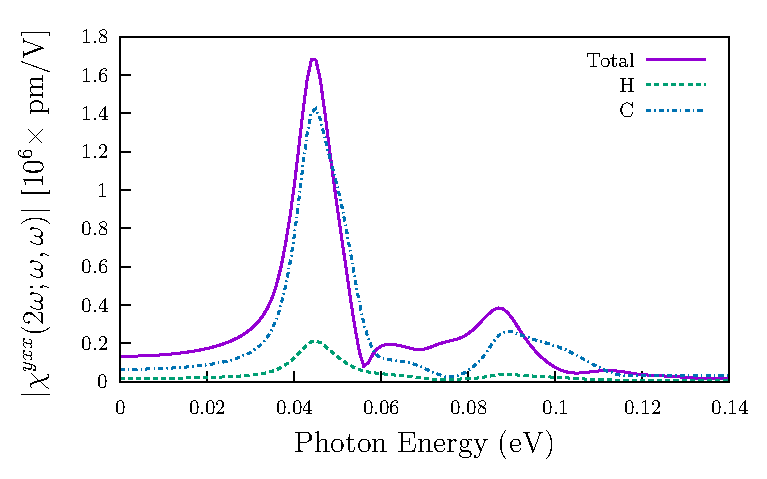
\includegraphics[width=\linewidth]{figures/shg-lay-up}}
\caption{(Color online) SHG spectra for the \emph{up} structure.
\label{fig:shg-vnl-up}}
\end{figure}

\begin{table}[htb]%
\centering
\sidecaption
\begin{tabular}{lcccc}
\hline
\hline
Structure & \hspace{-5mm}Energy & \multicolumn{2}{c}{$\chi^{abc} $} &  Ref.\\
\cline{3-4} & \hspace{-5mm}[eV] & $abc$ & value \\
\hline
C$_{16}$H$_{8}$-up    &  0.04  & yxx   & $1.7\times10^{6}$ \scriptsize{pm/V}  & *     \\
C$_{16}$H$_{8}$-alt   &  0.44  & xyy   & $3\times10^{3}$\,\scriptsize{pm/V}  & *     \\
Si(100)2$\times$1     &  1.82  & xxx   & 660\, \scriptsize{pm/V}  & \cite{andersonPRB15}  \\
BNNT(6,0) pristine    &  5.00  & zzz   & 35\,  \scriptsize{pm/V}  & \cite{salazarPRB14} \\
BNNT(6,0)+4(H$_{2}$)  &  5.00  & zzz   & 33\,  \scriptsize{pm/V}  & \cite{salazarPRB14} \\
BNNT(6,0)+12(H$_{2}$) &  4.80  & zzz   & 15\,  \scriptsize{pm/V}  & \cite{salazarPRB14} \\
\hline
\hline
\end{tabular}
\caption[]{%
Comparison of the highest reported absolute values of SHG for 
different structures and components. ($^{*}$This work)}
\label{tab:shgcomp}
\end{table}


\section{Conclusions}\label{sec:conclusions}

We have performed \emph{ab initio} calculations for the DSP, optical current
injection, and SHG on C$_{16}$H$_{8}$-alt and C$_{16}$H$_{8}$-up hydrogenated
graphene structures. The DSP, optical current injection, and SHG response are
very sensitive to the symmetry characteristics of the structures presenting an
anisotropic behavior. We found that it is possible induce DSP along the all
three Cartesian directions and we have that for the \emph{alt} structure the
absolute magnitude $\mathcal{D}(\omega)=61\%$ fixed at $\varphi=-46^{\circ}$ and
$\theta=35^{\circ}$ for a frequency of 0.72\,eV. For the \emph{up} structure we
found that it presents an absolute magnitude $\mathcal{D}(\omega)=64\%$ in the
fixed angles $\varphi=-18^{\circ}$ and $\theta=-62^{\circ}$ for a frequency of
0.08\,eV. According to this results both structures are good candidates for
spintronics applications. The energy values for the \emph{alt} and \emph{up}
structures make them interesting candidates for further study, as this energy is
readily obtainable using terahertz radiation.

For the optical current injection with circularly polarized light we found
that $\eta^{axy}(\omega)$ has components in the all three Cartesian directions
for an incoming circularly polarized light beam propagating along the $-z$
direction. For the \emph{alt} structure we found that the absolute current
injection magnitude is
$\eta(\omega)=5.10\,\mathrm{mC}^{3}/\mathrm{J}^{2}\mathrm{s}^{2}$ fixed at the
angles $\varphi=116^{\circ}$ and $\theta=-172^{\circ}$ for a photon energy of
0.97\,eV and for the \emph{up} system the absolute current injection magnitude
is $\eta(\omega)=15.12\,\mathrm{mC}^{3}/\mathrm{J}^{2}\mathrm{s}^{2}$ fixed at
the angles $\varphi=58^{\circ}$ and $\theta=-54^{\circ}$. Finally dealing with
the SHG we found that both structures are efficient to produce this phenomenon.
The highest value for the \emph{alt} structure is for the
$|\chi^{xyy}(-2\omega;\omega,\omega)|$ reaching a value near to
$3\times10^{3}\,\mathrm{pm/V}$ and the highest value for the \emph{up} structure
correspond to the $|\chi^{yxx}(-2\omega;\omega,\omega)|$ component reaching a
value of $1.7\times10^{6}\,\mathrm{pm/V}$. From this we conclude that
the \emph{up} structure is specially excellent for SHG.


\section{Acknowledgment} % (fold)

This work has been supported by \emph{Consejo Nacional de Ciencia y
Tecnolog\'ia} (CONACyT), M\'exico, Grant No. 153930.


\bibliographystyle{pss}
\bibliography{graphane_structures}

\end{document}
